
Front End languages are language that are used to give better user experince and user interface. These mainly include HTML, CSS, Javascript. Some Frameforks like Bootstrap are also used with these basic languages.
\subsection{HTML}

\begin{figure}[h]
\centering 
\includegraphics[scale=0.05]{images/HTML.png}
\caption{HTML5 logo}
\end{figure}
HyperText Markup Language, commonly referred to as HTML, is the standard markup language used to create web pages. Along with CSS, and JavaScript, HTML is a cornerstone technology, used by most websites to create visually engaging webpages, user interfaces for web applications, and user interfaces for many mobile applications. Web browsers can read HTML files and render them into visible or audible web pages. HTML describes the structure of a website semantically along with cues for presentation, making it a markup language, rather than a programming language.


HTML elements form the building blocks of all websites. HTML allows images and objects to be embedded and can be used to create interactive forms. It provides a means to create structured documents by denoting structural semantics for text such as headings, paragraphs, lists, links, quotes and other items.

\begin{verbatim}
<!DOCTYPE html>
<html>
  <head>
    <title>This is a title</title>
  </head>
  <body>
    <p>Hello world!</p>
  </body>
</html>

\end{verbatim}


\subsection{CSS}

\begin{figure}[h]
\centering 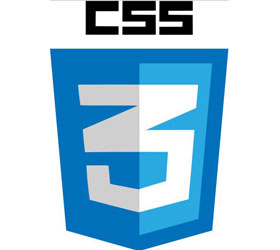
\includegraphics[scale=0.50]{images/CSS.jpg}
\caption{CSS logo}
\end{figure}
Cascading Style Sheets (CSS) is a style sheet language used for describing the presentation of a document written in a markup language.Although most often used to set the visual style of web pages and user interfaces written in HTML and XHTML, the language can be applied to any XML document, including plain XML, SVG and XUL, and is applicable to rendering in speech, or on other media. Along with HTML and JavaScript, CSS is a cornerstone technology used by most websites to create visually engaging webpages, user interfaces for web applications, and user interfaces for many mobile applications.


CSS is designed primarily to enable the separation of document content from document presentation, including aspects such as the layout, colors, and fonts. This separation can improve content accessibility, provide more flexibility and control in the specification of presentation characteristics, enable multiple HTML pages to share formatting by specifying the relevant CSS in a separate .css file, and reduce complexity and repetition in the structural content, such as semantically insignificant tables that were widely used to format pages before consistent CSS rendering was available in all major browsers. CSS makes it possible to separate presentation instructions from the HTML content in a separate file or style section of the HTML file. For each matching HTML element, it provides a list of formatting instructions

\begin{verbatim}
p {
    color: red;
    text-align: center;
} 
\end{verbatim}

\subsection{Javascript}
\begin{figure}[h]
\centering 
\includegraphics[scale=0.3]{images/JS.png}
\caption{Javascript logo}
\end{figure}
JavaScript (/ˈdʒɑːvəˌskrɪpt/) is a high-level, dynamic, untyped, and interpreted programming language. It has been standardized in the ECMAScript language specification. Alongside HTML and CSS, it is one of the three essential technologies of World Wide Web content production; the majority of websites employ it and it is supported by all modern web browsers without plug-ins. JavaScript is prototype-based with first-class functions, making it a multi-paradigm language, supporting object-oriented, imperative, and functional programming styles. It has an API for working with text, arrays, dates and regular expressions, but does not include any I/O, such as networking, storage or graphics facilities, relying for these upon the host environment in which it is embedded.

\subsection{BootStarp} 
\begin{figure}[h]
\centering 
\includegraphics[scale=0.2]{images/boot.png}
\caption{BootStrap logo}
\end{figure}

Bootstrap is a free and open-source collection of tools for creating websites and web applications. It contains HTML and CSS-based design templates for typography, forms, buttons, navigation and other interface components, as well as optional JavaScript extensions. It aims to ease the development of dynamic websites and web applications.

Bootstrap is a front end framework, that is, an interface for the user, unlike the server-side code which resides on the "back end" or server.


